\chapter{实验结果及分析}
\label{chap:experiment}

\section{分子生成}

\subsection{实验设置}
在本节中,我们报告了GFMDiff在两个主流数据集GEOM-QM9 \cite{qm9_ramakrishnan_14}和GEOM-Drugs \cite{drugs_axelrod_22}上的性能。结果表明,我们的方法在多个方面显著优于一些最先进的模型。

为了进行全面的比较,我们在两个分子生成的基准数据集上进行了实验:GEOM-QM9 \cite{qm9_ramakrishnan_14}和GEOM-Drugs \cite{drugs_axelrod_22}。GEOM-QM9数据集包含超过130K个分子及其对应的构象,其中平均每个分子有18个原子,包括氢原子。GEOM-Drugs是一个规模较大的数据集,包括的分子数量和平均分子数量都较多。它包含超过450K个分子和37M个构象,其中平均分子大小为44。

\subsection{在GEOM-QM9数据集上的全新三维分子生成}


\begin{table}[h]
    \centering
    \caption{GEOM-QM9上分子生成结果对比表}
    \label{tab:exp_qm9}
    \begin{tabular}{llllll}
    \hline
    Method & NLL$\downarrow$ & \makecell[l]{Atom\\Stable\\(\%) $\uparrow$} & \makecell[l]{Mol\\Stable\\(\%) $\uparrow$} & \makecell[l]{Valid\\(\%) $\uparrow$} & \makecell[l]{Unique$\cdot$Valid\\(\%) $\uparrow$} \\
    \hline
    E-NF & -59.7 & 85.0 & 4.9 & 40.2 & 39.4 \\
    G-SchNet & N/A & 95.7 & 68.1 & 85.5 & 80.3 \\
    EDM & -110.7$\pm$1.5 & 98.7$\pm$0.1 & 82.0$\pm$0.4 & 91.9$\pm$0.5 & 90.7$\pm$0.6 \\
    Bridge & N/A & 98.7$\pm$0.1 & 81.8$\pm$0.2 & N/A & N/A \\
    Bridge+Force & N/A & \underline{98.8}$\pm$0.1 & 84.6$\pm$0.3 & N/A & N/A \\
    GCDM & \textbf{-171.0}$\pm$0.2 & 98.7$\pm$0.0 & 85.7$\pm$0.4 & 94.8$\pm$0.2 & 93.3$\pm$0.0 \\
    \hline
    \makecell[l]{GFMDiff\\w/o tri} & -123.1$\pm$0.4 & 98.7$\pm$0.1 & 85.9$\pm$0.2 & 94.9$\pm$0.2 & 94.2$\pm$0.2 \\
    \makecell[l]{GFMDiff\\w/o GFLoss} & -127.5$\pm$0.4 & 98.7$\pm$0.0 & \underline{86.5}$\pm$0.1 & \underline{95.2}$\pm$0.0 & \underline{94.5}$\pm$0.0 \\
    GFMDiff & \underline{-128.0}$\pm$0.2 & \textbf{98.9}$\pm$0.0 & \textbf{87.7}$\pm$0.2 & \textbf{96.3}$\pm$0.3 & \textbf{95.1}$\pm$0.2 \\
    \hline
    Data &  & 99.0 & 95.2 & 97.7 & 97.7 \\
    \hline
    \end{tabular}
\end{table}
\begin{figure}[h]
    \centering
    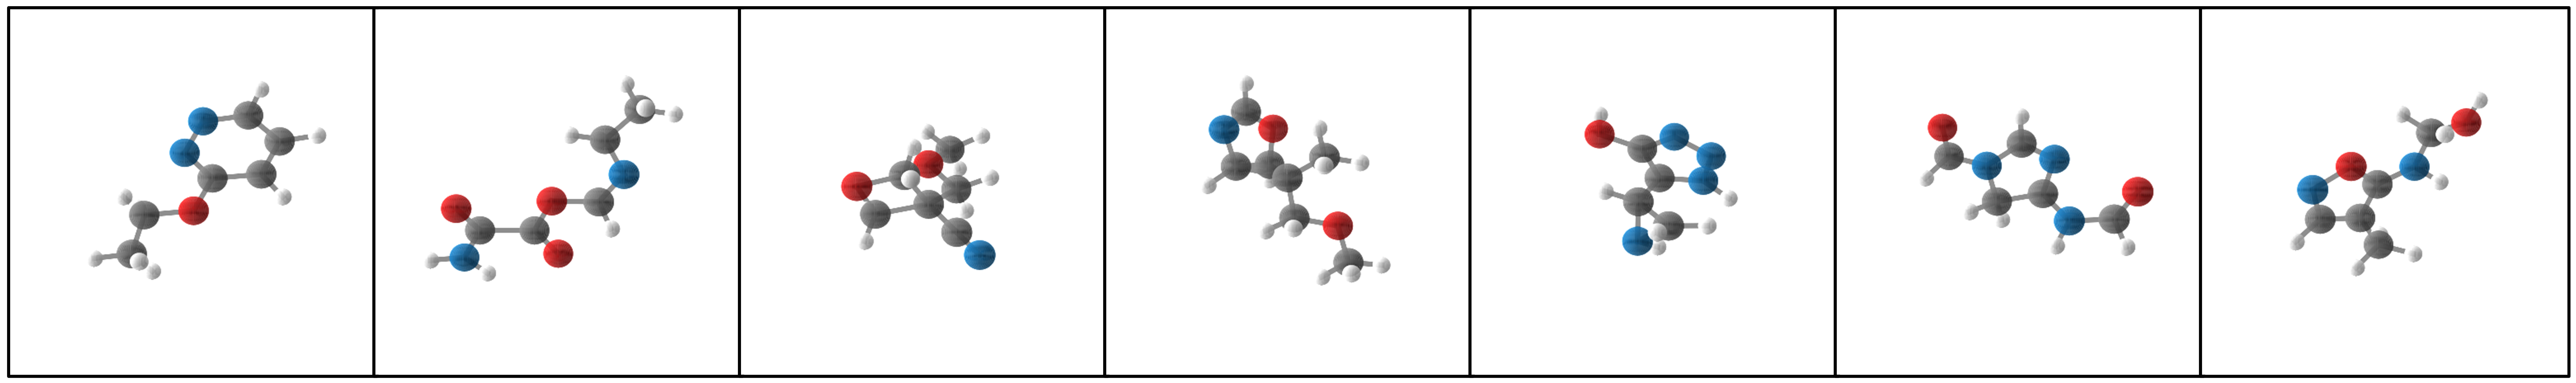
\includegraphics[width=\linewidth]{figures/samples_qm9.png}
    \caption{GEOM-QM9上分子生成样本示意图}
    \label{fig:samples_qm9}
\end{figure}

\subsection{在GEOM-QM9数据集上的条件三维分子生成}

\begin{table}[H]
    \centering
    \caption{GEOM-QM9上分子条件生成结果对比表}
    \label{tab:exp_qm9_condition}
    \begin{tabular}{lllllll}
    \hline
    \makecell[l]{Task\\Units} & \makecell[l]{$\alpha$\\${\rm Bohr^3}$} & \makecell[l]{$\Delta \varepsilon$\\${\rm meV}$} & \makecell[l]{$\varepsilon_{{\rm HOMO}}$\\${\rm meV}$} & \makecell[l]{$\varepsilon_{{\rm LUMO}}$\\${\rm meV}$} & \makecell[l]{$\mu$\\${\rm D}$} & \makecell[l]{$C_v$\\$\frac{{\rm cal}}{{\rm mol}}{\rm K}$} \\
    \hline
    Naive (Upper-bound) & 9.01 & 1470 & 645 & 1457 & 1.616 & 6.857 \\
    \# Atom & 3.86 & 866 & 426 & 813 & 1.053 & 1.971 \\
    EDM & 2.76 & 655 & 356 & 584 & 1.111 & 1.101 \\
    GCDM & \underline{1.97} & \underline{602} & \underline{344} & \underline{479} & \underline{0.844} & \underline{0.689} \\
    GFMDiff & \textbf{1.74} & \textbf{558} & \textbf{321} & \textbf{430} & \textbf{0.728} & \textbf{0.593} \\
    QM9 (Lower-bound) & 0.10 & 64 & 39 & 36 & 0.043 & 0.040 \\
    \hline
    \end{tabular}
\end{table}
\begin{figure}[H]
    \centering
    \includegraphics[width=\linewidth]{figures/samples_qm9_cond.png}
    \caption{GEOM-QM9上分子条件生成样本示意图}
    \label{fig:samples_qm9_cond}
\end{figure}


\subsection{在GEOM-Drugs数据集上的三维分子生成}

\begin{table}[h]
    \centering
    \caption{GEOM-Drugs上分子生成结果对比表}
    \label{tab:exp_drugs}
    \begin{tabular}{llll}
    \hline
    Type & Method & Atom Stable (\%) $\uparrow$ & Mol Stable (\%) $\uparrow$ \\
    \hline
    Normalizing flow & E-NF & 75.0 & 0 \\
    \multirow{2}{*}{DDPM}
    & EDM  & 81.3 & 0.0 \\
    & Bridge & 81.0$\pm$0.7 & 0.0 \\
    & Bridge+Force & 82.4$\pm$0.8 & 0.0 \\
    & GCDM & 86.4$\pm$0.2 & 3.7$\pm$0.3 \\
    \hline
    Ours & GFMDiff & \textbf{86.5}$\pm$0.2 & \textbf{3.9}$\pm$0.2 \\
    \hline
    Data &  & 86.5 & 2.8 \\
    \hline
    \end{tabular}
\end{table}
\begin{figure}[h]
    \centering
    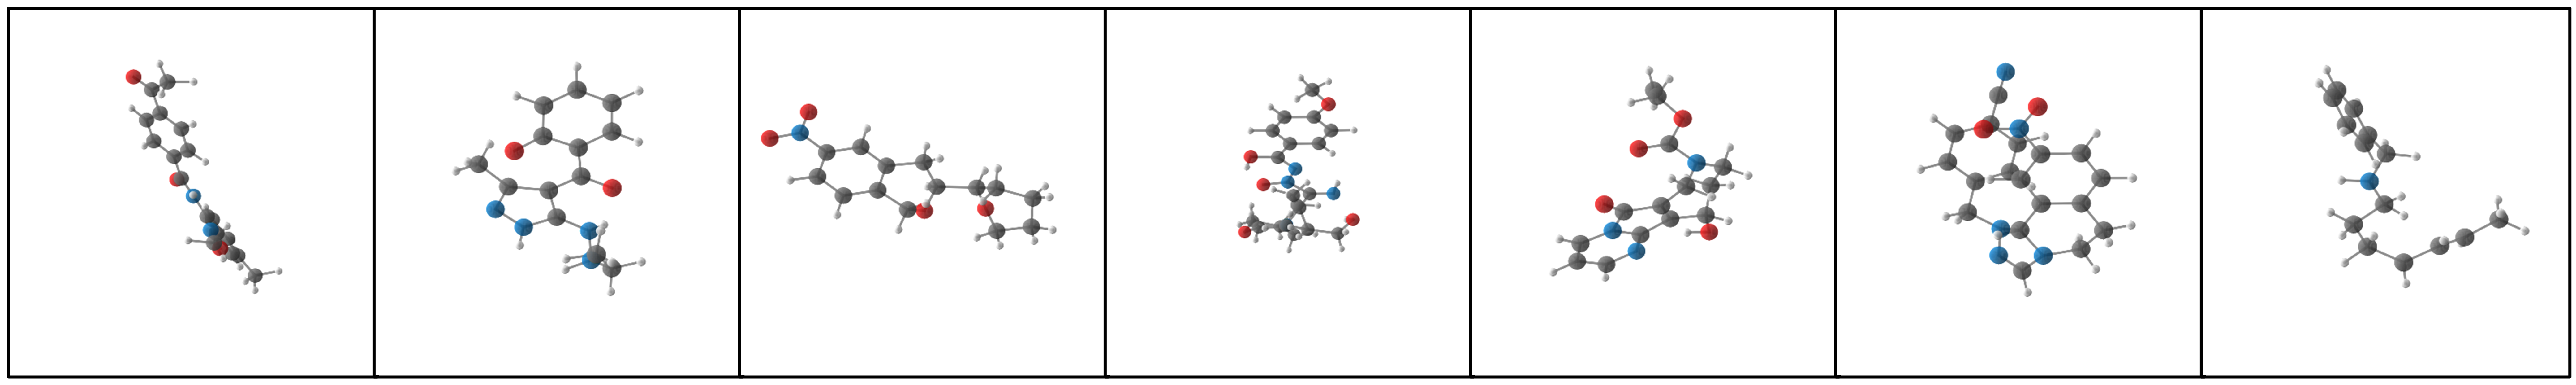
\includegraphics[width=\linewidth]{figures/samples_drugs.png}
    \caption{GEOM-Drugs上分子生成样本示意图}
    \label{fig:samples_drugs}
\end{figure}

\section{分子性质预测}

\subsection{实验设置}

\subsection{在GEOM-QM9数据集上的分子性质预测}

\begin{table}[h]
    \centering
    \caption{Performance comparison on QM9}
    \label{tab:exp_qm9_reg}
    \begin{tabular}{lllllll}
    \hline
    \makecell[l]{Task\\Units} & \makecell[l]{$\alpha$\\${\rm Bohr^3}$} & \makecell[l]{$\Delta \varepsilon$\\${\rm meV}$} & \makecell[l]{$\varepsilon_{{\rm HOMO}}$\\${\rm meV}$} & \makecell[l]{$\varepsilon_{{\rm LUMO}}$\\${\rm meV}$} & \makecell[l]{$\mu$\\${\rm D}$} & \makecell[l]{$C_v$\\$\frac{{\rm cal}}{{\rm mol}}{\rm K}$} \\
    \hline
    Naive (Upper-bound) & 9.01 & 1470 & 645 & 1457 & 1.616 & 6.857 \\
    \# Atom & 3.86 & 866 & 426 & 813 & 1.053 & 1.971 \\
    EDM & 2.76 & 655 & 356 & 584 & 1.111 & 1.101 \\
    GCDM & 1.97 & 602 & 344 & 479 & 0.844 & 0.689 \\
    GeoDiff &  &  &  &  &  & \\
    QM9 (Lower-bound) & 0.10 & 64 & 39 & 36 & 0.043 & 0.040 \\
    \hline
    \end{tabular}
\end{table}

\subsection{在OC20数据集上的分子性质预测}
